\documentclass[11 pt]{llncs}
%\documentclass{sig-alternate}
% -------------defined commands------------
%\newcommand{\creator}{creator}
%\newcommand{\sessionLabels}{slabel}
%\newcommand{\Policy}{Policy}
%
\newcommand{\PM}{\textit{PM}}
\newcommand{\LAP}{\textit{LAP}}
\newcommand{\EAP}{\textit{EAP}}
\newcommand{\TL}{\textit{TL}}
%
\newcommand{\userLabel}[1]{uLabel_{#1}}
\newcommand{\objectLabel}[1]{oLabel_{#1}}
%\newcommand{\UL}[1]{UL_#1}
%\newcommand{\OL}[1]{OL_#1}
%\newcommand{\userLabelOne}{$uLabel_1$}
%
%
%%---------EP-ABAC Models---------------%
\newcommand{\EPModels}{$EAP$-$ABAC$}
\newcommand{\EPZeroOneOne}{$EP_{0}$-$ABAC^{1,1}$}
\newcommand{\EPHOneOne}{$EP_{H}$-$ABAC^{1,1}$}
\newcommand{\EPSOneOne}{$EP_{S}$-$ABAC^{1,1}$}
\newcommand{\EPPMOneOne}{$EP_{\pm}$-$ABAC^{1,1}$}
\newcommand{\EPOneOneModels}{$EP$-$ABAC^{1,1}$}
\newcommand{\EPMNModels}{$EP$-$ABAC^{m,n}$}
%
%\newcommand{\EPZeroOneOne}{\clabac}
%\newcommand{\EPHOneOne}{\hlabac}
%\newcommand{\EPSOneOne}{\slabac}
%\newcommand{\EPPMOneOne}{\npLabac}
%\newcommand{\EPOneOneModels}{$EAP$-$ABAC_{1,1}$}
\newcommand{\EPMNModel}{$EAP$-$ABAC_{m,n}$}
%
%
\newcommand{\LPModels}{$LAP$-$ABAC$}
\newcommand{\LPOneOne}{$LAP$-$ABAC_{1,1}$}
\newcommand{\LPMN}{$LAP$-$ABAC_{m,n}$}
\newcommand{\pmlabac}{$LaBAC_{\pm}^{1,1}$}
%
%% ---------------Other models-----------------
%\newcommand{\abacAlpha}{ABAC_\alpha}
%\newcommand{\hgabac}{$HGABAC$}
%\newcommand{\twoSortedRBAC}{2-sorted-RBAC}
%
%% ------------Higher Level LABAC---------------
%
%\newcommand{\labacOneTwoTwo}{$LaBAC_{1}^{2,2}$}
%\newcommand{\labacOneOneOne}{$LaBAC_{1}^{1,1}$}
%\newcommand{\labacOneMN}{$LaBAC_{1}^{m,n}$}
%\newcommand{\labacZeroMN}{$LaBAC_{0}^{m,n}$}
%\newcommand{\setLabac}{$LaBAC_{S}^{1,1}$}
%
%\newcommand{\labacNPMN}{$LaBAC_{\pm}^{m,n}$}
%\newcommand{\abacOneOne}{$LP$-$ABAC^{1,1}$}
%\newcommand{\labacOneOne}{$LaBAC^{1,1}$}
%
%%--------- LaBAC Names -----
%\newcommand{\labac}{$LaBAC$}
%\newcommand{\clabac}{$LaBAC_{0}^{1,1}$}
%\newcommand{\hlabac}{$LaBAC_{H}^{1,1}$}
%\newcommand{\slabac}{$LaBAC_{S}^{1,1}$}
%\newcommand{\npLabac}{$LaBAC_{\pm}^{1,1}$}
%\newcommand{\consLabac}{$LaBAC_{C}^{1,1}$}
%\newcommand{\elabac}{$LaBAC_{E}^{1,1}$}
%\newcommand{\labacOneOneFamily}{$LaBAC^{1,1}$}
%
%
%%------------LaBAC administrative ops-------------%
%\newcommand{\policyReview}{policy\_review}
%
%
%%-------------------- LaBAC Components-----------------
%\newcommand{\uLabel}{uLabel}
%\newcommand{\oLabel}{oLabel}
%\newcommand{\uLabelOne}{uLabel_1}
%\newcommand{\oLabelOne}{oLabel_1}
%\newcommand{\uLabelTwo}{uLabel_2}
%\newcommand{\oLabelTwo}{oLabel_2}
%\newcommand{\canAddPolicy}{can\_manage\_policy}
%\newcommand{\lb}{ }
%\newcommand{\OBJ}{O}
%\newcommand{\objmem}{o}
%\newcommand{\U}{U}
%\newcommand{\umem}{u}
%\newcommand{\amem}{a}
%\newcommand{\A}{A}
%
%\newcommand{\OLV}{OL}
%\newcommand{\olvmem}{ol}
%\newcommand{\ULV}{UL}
%\newcommand{\ulvmem}{ul}
%\newcommand{\OLA}{OLA}
%\newcommand{\ULA}{ULA}
%\newcommand{\OLH}{OLH}
%\newcommand{\ULH}{ULH}
%
%\newcommand{\policy}{Policy}
%\newcommand{\odominate}{\succeq_{ol}}
%\newcommand{\udominate}{\succeq_{ul}}
%\newcommand{\impliedPolicy}{Implied\_policy}
%\newcommand{\effectivePolicy}{Effective\_policy}
%\newcommand{\policyBound}{ValidPolicy}
%
%\newcommand{\maxPolicy}{|policy|_{max}}
%\newcommand{\maxPolicySet}{|\policy|_{max}}
%\newcommand{\request}{is\_authorized}
%
%
%% -------------session command------------
%\newcommand{\addSessionLabels}{add\_session\_labels}
%\newcommand{\removeSessionLabels}{remove\_session\_labels}
%\newcommand{\addSessionValues}{add\_session\_values}
%\newcommand{\removeSessionValues}{remove\_session\_values}
%\newcommand{\createSession}{create\_session}
%\newcommand{\deleteSession}{delete\_session}
%\newcommand{\createSubject}{create\_subject}
%\newcommand{\deleteSubject}{delete\_subject}
%\newcommand{\assignValues}{assign\_values}
%\newcommand{\removeValues}{remove\_values}
%
%%------------------ABAC^11 commands--------------
%
\newcommand{\UAV}[1]{\textit{UAV}_{#1}}
\newcommand{\OAV}[1]{\textit{OAV}_{#1}}
\newcommand{\ua}[1]{ua_{#1}}
\newcommand{\sa}[1]{sa_{#1}}
\newcommand{\oa}[1]{oa_{#1}}
\newcommand{\subCreator}{creator}
\newcommand{\uLabelP}[1]{\uLabel_{#1}}
\newcommand{\oLabelP}[1]{\oLabel_{#1}}
\newcommand{\ULS}[1]{ULS_{#1}}
\newcommand{\OLS}[1]{OLS_{#1}}
\newcommand{\val}[1]{\textit{Val}_{#1}}
\newcommand{\uVal}[1]{\textit{uVal}_{#1}}
\newcommand{\oVal}[1]{\textit{oVal}_{#1}}
\newcommand{\sessionLabelsP}[1]{\sessionLabels_{#1}}


%---------------ABAC, labac equivalence commands------------

\newcommand{\isAuthorized}{is\_authorized}
\newcommand{\GammaLabac}{\Gamma^{L}}
\newcommand{\gammaLabac}{\gamma^{L}}
\newcommand{\GammaA}{\Gamma^{A}}
\newcommand{\gammaA}{\gamma^{A}}
\newcommand{\GammaB}{\Gamma^{L}}
\newcommand{\gammaB}{\gamma^{L}}
\newcommand{\QLabac}{Q^{L}}
\newcommand{\qLabac}{q^{L}}
\newcommand{\QA}{Q^{A}}
\newcommand{\qA}{q^{A}}
\newcommand{\QB}{Q^{L}}
\newcommand{\qB}{q^{L}}
\newcommand{\qs}{q_s^{L}}
\newcommand{\qsa}{q_s^{A}}

\newcommand{\vdashA}{\vdash^{A}}
\newcommand{\vdashB}{\vdash^{L}}
\newcommand{\vdashLabac}{\vdash^{L}}
\newcommand{\GammaABAC}{\Gamma^{A}}
\newcommand{\gammaABAC}{\gamma^{A}}
\newcommand{\QABAC}{Q^{A}}
\newcommand{\qABAC}{q^{A}}
\newcommand{\vdashABAC}{\vdash^{A}}
\newcommand{\PABAC}{P^A}
\newcommand{\PLabac}{P^L}
\newcommand{\qal}{q_{aij}^L}
\newcommand{\qaa}{q_{aij}^A}
\newcommand{\ulpm}{UL_{\pm} }
\newcommand{\olpm}{OL_{\pm} }
\newcommand{\ulsubset}{UL_i}
\newcommand{\olsubset}{OL_j}
\newcommand{\gammaStartLabac}{\gamma_{0}^{L}}
\newcommand{\gammaStartABAC}{\gamma_{0}^{A}}
\newcommand{\gammaKLabac}{\gamma_{k}^{L}}
\newcommand{\gammaKABAC}{\gamma_{k}^{A}}

\newcommand{\mapping}{\overset{*}{\longmapsto_\psi}}
\newcommand{\mappingABAC}{\overset{*}{\longmapsto_{\psi_{A}}}}

%--------Tripli Commands ---------------
\newcommand{\mygamma}[2]{\gamma_{#1}^{#2}}
\newcommand{\myGamma}[1]{\Gamma^{#1}}
\newcommand{\mylongmapsto}[1]{\overset{*}{\longmapsto_#1}}
%\newcommand{\myVdash}{1}{\vdash^{#1}}
\newcommand{\myvdash}[1]{\vdash^{#1}}

\newcommand{\myq}[2]{q_{#1}^{#2}}
\newcommand{\myQ}[1]{Q^{#1}}
\newcommand{\myPSI}[1]{\Psi^{#1}}


%----------policy review functions---------


\newcommand{\subsetUL}{UL_s}
\newcommand{\subsetOL}{OL_s}
\newcommand{\setULs}{2^{UL}}
\newcommand{\setOLs}{2^{OL}}

%---------Tripli equivalence functions----------
\newcommand{\smallGamma}[1]{\gamma^{#1}}
\newcommand{\bigGamma}[1]{\Gamma^{#1}}
\newcommand{\smallQ}[1]{q_{s}^{#1}}
\newcommand{\bigQ}[1]{Q^{#1}}
\newcommand{\bigVdash}[1]{\vdash^{#1}}
\newcommand{\smallPsi}[1]{\psi^{#1}}
\newcommand{\bigPsi}[1]{\Psi^{#1}}

\newcommand{\curModelSymbol}{Z}
\newcommand{\manager}{mng}


\usepackage[utf8]{inputenc}
\usepackage{caption}
\usepackage{graphicx}
\usepackage{amsmath}
\usepackage{xcolor}
\usepackage{underscore}
\usepackage{epstopdf}
\epstopdfsetup{outdir=./}

\begin{document}

\pagenumbering{arabic}


%\title{On design and characterization of expressive powers of an enumerated policy finite domain ABAC model}
%\title{On design and analysis of expressive power of finite domain enumerated authorization policy ABAC models}
%\title{On Expressive Power of Enumerated Authorization Policy ABAC Models in Finite Domain}
%\title{On comparison of Finite Domain Logical-formula and Enumerated Authorization Policy ABAC Models in Expressive Power and Beyond}
%\title{On Expressive Power and Beyond of Logical-formula and Enumerated Authorization Policy ABAC Models in Finite Domain}
\title{A Comparison of Logical-formula and Enumerated Authorization Policy ABAC Models}


\date{30 July 1999}

\maketitle

\begin{abstract}
	
 There has been considerable research in specifying authorization policies for XML documents. Most of these approaches consider only \textit{hierarchical structure} of underlying data. They define authorization policies by directly identifying XML nodes in the policies. These approaches work well for hierarchical structure but are not suitable for other required characteristics we identify in this paper as \textit{semantical association} and \textit{scatteredness}.
 
 
This paper presents an attribute based protection model for JSON documents. We assign \textit{security-label} attribute values  to JSON elements and specify authorization policies using these values. By using security-label attribute, we leverage  semantical association and scatteredness properties. Our protection mechanism defines two types of policies called  authorization and labeling policies. We present an operational model to specify authorization policies and  different models for defining labeling policies. Finally, we demonstrate a proof-of-concept for the proposed models in the Swift service of OpenStack IaaS cloud.

% In our approach, we assign \textit{security-label} attribute values  to JSON elements in a JSON document and specify authorization policies using these attribute values. Thus, our protection model have a  level of indirection where JSON objects are first annotated with security-label values which can  be managed independently from the JSON documents and seamlessly with other higher level organizational policies. We lay out an architecture of our protection model and  specify labeling policies to assign attribute values to JSON objects. Our protection model is significantly different than most of the existing XML protection models which directly assign authorization policies on XML nodes. These models (XML models) may result duplicated authorization policies which are hard to manage or administer. We believe, our protection model can also be used for XML data as well.


% and Our protection model is significantly different than most of the existing XML protection models which could have been  adopted for protecting JSON documents. In this perspective, we argue that most of the existing protection models for XML directly assign authorization policies on XML nodes which leaves the possibility of duplicated authorization policies for similar (in term of authorization requirement) but different information. 


 %While XML and JSON 
	
%JSON or JavaScript Object Notation is an open standard for data interchange which is gaining immense popularity due to its concise representation and ease of human and machine readability. Industries are increasingly adopting JSON for internal data representation and data transfer format which is reflected by developments including JSON  document database such as MongoDB (more accurately BSON, a modified version JSON) is now officially supported by the OpenStack cloud platform, Twitter latest API (v 1.1) supports only JSON and YouTube latest API (v 3) recommends JSON as the default exchange format. Interestingly, in spite of industry demand, JSON has received minimal interest from the research community.

%In this paper, we investigate access control scope for JSON documents. We present a label based protection mechanism for JSON data. For this purpose, we have demonstrated a simple label based access control model and shown different ways (path based, content based and attribute based) of labeling JSON items automatically or semi-automatically to reduce labeling efforts. We have also specified label based constraints to capture practical labeling requirements. We have implemented the protection mechanism for JSON documents stored as OpenStack Swift objects. As part of our implementation, we have extended ACL based `all or nothing' access of a Swift object towards content level partial access.

%We present a simple attribute based access control model for this purpose and demonstrate a corresponding protection mechanism.  To the best of our knowledge, we are the first to attempt this kind of work for JSON documents. We have implemented  our proposed access control model and made it available as a standard package in the official Python repository.
\end{abstract} 
\chapter{Introduction}






\section{Motivation}




\section{Problem statement and thesis}
\subsection{Problem statement}
There are two major techniques for specifying authorization policies in Attribute Based Access Control (ABAC). The more conventional approach is to define policies using logical formulas involving attribute values. The alternate technique is by enumeration. While considerable work has been done for the former approach, the later  lacks fundamental work from the research community.

\subsection{Thesis}
\textit{Enumerated Authorization Policy ABAC (EAP-ABAC) model is a viable alternate to Logical-formula Authorization Policy ABAC (LAP-ABAC) model. EAP-ABAC is as expressive as LAP-ABAC in the finite domain. EAP-ABAC models can be enforced in different application domains.}


\section{Summary of contribution}

\section{Organization of the dissertation}


\chapter{Background \& Literature Review}

\section{Finite Domain ABAC}
	Most of the ABAC models (for example, \cite{abacAlpha,hgabac,abac-ws,abac-for-web-service}) assume finite set of user and  object attributes and that values of each attribute come from a finite set. This assumption is useful in many practical cases. For example, values of \textit{roles}, \textit{clearance} or \textit{age} are bounded and mostly static. But attribute values can be unbounded as well. For example, if values of an attribute include users or objects in a system  (e.g. \textit{owner} of an object) where they may grow indefinitely, these values are unbounded.  In this dissertation, we assume that there is a finite set of attributes and values of each attribute come from a finite set.
	
\section{Types of authorization policy}
	Most of the ABAC models assume a finite set of user attributes, finite set of object attributes and finite range for each of these attribute functions. On the other hand, when specifying authorization policies, there are two major methods. More conventional approach is to define policies using logical formula. Examples in this category include $\abacAlpha${} \cite{abacAlpha}, \hgabac{} \cite{hgabac}, ABAC for Web Services \cite{abac-for-web-service}, and XACML \cite{xacml}. The alternative technique for expressing policy is by enumeration. Examples in this category include Policy Machine (PM) \cite{policy-machine} and \twoSortedRBAC{} \cite{two-sorted-rbac}.
	
\subsection{Logical-formula Authorization policy}
	Logical-formula authorization policy (\LAP{}) can be defined as a boolean expression consisting of subexpressions connected with logical operators (for example, $\land, \lor, \lnot$ and so on ) where each subexpression compares attribute values with other attribute or constant values. The language for \LAP{} usually supports a large set of logical and relational operators. A \LAP{} grants a user request for exercising certain action on an object if attributes of the requesting user and requested object evaluate the formula true. $Auth_{read} \equiv clearance(u) \succeq classification(o)$ is an example of  logical-formula authorization policy which allows a user to read an object if the user's clearance dominates classification of the object.
	
	\LAP{}s are usually expressed in propositional logic. Examples of  \LPModels{} models  include \cite{abacAlpha,hgabac,abac-ws,abac-for-web-service}.  Flexibility of these models have been demonstrated by configuring conventional DAC\cite{dac}, MAC\cite{lbac} and RBAC \cite{rbac} policies in it. 
	
	%It has been shown  \cite{labac} that policy review in  \LPModels{} is equivalent to the satisfiability problem  which is NP-complete for propositional logic. 
	
	As satisfiability in propositional logic is NP-complete and policy review in general can be mapped to satisfiability problem, reviewing policy would be NP-Complete in many existing ABAC models including \cite{abacAlpha,hgabac,abac-for-web-service}. On the other hand, if policies are expressed in first-order logic, policy review would be undecidable since  satisfiability is undecidable in first-order logic.
	
\subsection{Enumerated Authorization Policy}
	Usefulness of enumerated authorization policy has been demonstrated in the literature. For example, in Policy Machine (PM) \cite{policy-machine}, Ferraiolo et. al define attribute based enumerated policies using one user attribute, one object attribute and a set of actions. A policy/privilege in PM is defined as $(ua_i, OP, oa_i)$, where $ua_i$ and $oa_i$ are values of user-attribute and object-attribute respectively and $OP$ is  a set of operations. Intuitively, reviewing or updating an enumerated policy would be polynomial time.
		
	The simple structure of enumerated policy does not necessarily make it less expressive. For example, PM shows how to configure traditional models using enumerated policies \cite{INCITS526}. In Section \ref{sec:configuration}, we also show how to express RBAC \cite{rbac} and LBAC \cite{lbac} policies using \EAP{}s. Furthermore, in Section \ref{sec:equivalence}, EAP and LAP are are equivalent in their theoretical expressive power.
	
	Informally, an enumerated authorization policy (\EAP{}) consists of a set of  tuples.  Each tuple \textit{(UAVals, OAVals)} grants privileges to a set of users  to exercise an action on a set of objects identified by the user and object attribute values \textit{UAVals} and \textit{OAVals} respectively. In an EAP, each tuple is distinct and grants privileges independently. Both  UAVals{} and OAVals{} can be atomic valued or set valued. (\textit{\manager, TS}) and (\textit{\{\manager, dir\}, \{TS,H\}}) are example of atomic and set valued tuples respectively. 
	
	

%\section{Theoretical expressive power}

\section{Literature Review}


Several attribute based access control models have been proposed in the literature. While, some authors design general purpose ABAC model, others design ABAC in specific application context. There are also significant works towards integrating attributes with traditional RBAC model for enhancing its expressibility. Furthermore, XACML represent another line of work involving attributes to provide flexible policy language and support of multiple access control policies.

$\abacAlpha${} \cite{abacAlpha} is among the first few models to formally define an ABAC model. It is designed to demonstrate flexibilities of an ABAC system to configure DAC, MAC and RBAC models. $\abacAlpha${} uses subset of subject attributes and object attributes to define  an authorization policy for a particular permission $p$. It describes a constraint language to specify subject attributes from user attributes. Furthermore, it also presents a constraint language for changing object attributes at  creation or modification time.

\hgabac{} \cite{hgabac} is another notable work in designing a formal model for an ABAC system. Besides designing a flexible policy language capable of  configuring DAC, MAC and RBAC, it also addresses a real problem of assigning attributes to a large set of users and objects. It specifies hierarchical groups and provides a mechanism for inheriting attributes from a group by joining to the group.

ABAC-for-web-services \cite{abac-for-web-service} is among very few earlier works to outline authorization architecture and policy formulation for an ABAC system. They propose a distributed architecture for authoring, administering, implementing and enforcing an ABAC system. Even though, their policy language is semi-formal, they present a powerful idea of composing hierarchical policies from individual policies.

Wang et al \cite{wang2004logic} presents a stratified logic programming based framework to specify ABAC policies. Even though, they only consider user attributes, they focus on providing a consistent, high performance and workable solution for ABAC system.



In its ABAC guide \cite{nist-abac-draft} and other publications \cite{hu2015attribute},  NIST defines common terminologies, and concepts for an ABAC system. It discusses required components, considerations and architecture for designing an  enterprise ABAC system. It acknowledges the fact that ABAC rules can be quite complex in boolean combination of attributes or in simple relations involving attributes. Additionally, it discusses more advanced features like attribute and policy engineering, federation of attributes and so on. Nonetheless, these documents are focused towards establishing general definitions and considerations of an ABAC system without providing a concrete model definition.

There are other works that design an ABAC system from a particular application context. For example, WS-ABAC \cite{abac-ws}  is motivated by requirements in web services, ABAC-in-grid \cite{grid-abac}  is motivated by needs in the grid computing.



Another interesting line of work combines attributes with Role Based Access Control. Kuhn et. al \cite{kuhn2010adding} provides a framework for combining roles and attributes. In the framework, they briefly outline three different approaches - (i) dynamic roles which retain basic structure or RBAC and  uses attribute based rules to derive user roles, (ii) attribute centric,  which treat role as another ordinary attribute, and (iii) role centric, which uses roles to grant permissions and attributes to reduce permissions to be available to the user. Various other earlier or subsequent works involving roles and attributes can also be cast in Kuhn's framework. For example, attribute-based user-role assignment by Al-Kahtani et. al \cite{al2002model} can be considered as an approach based on dynamic roles.

Last but not the least, XACML \cite{xacml} is a declarative access control policy language and processing model which  supports attribute based access control concepts and policies. Although, it lacks a formal definition of an ABAC model, it is notable for its uses in multiple commercial products.


	
	
 	\begin{figure} 
 		\centering
 		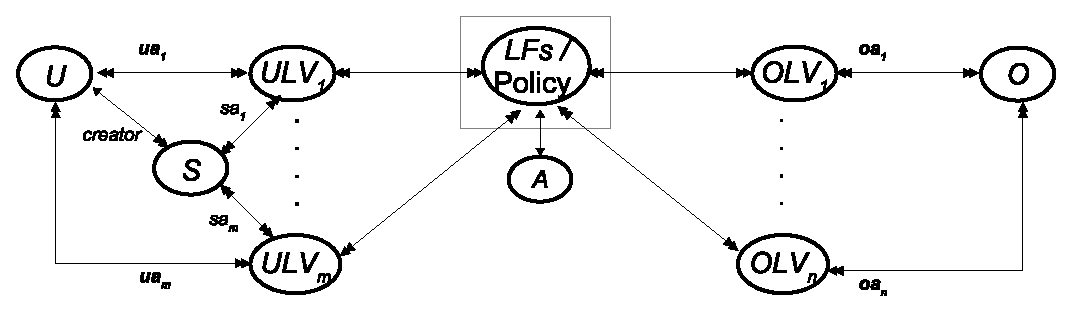
\includegraphics[width=.9\textwidth]{DBSEC16/lpabac-mn}
 		\caption{Components of \LPModels{} model with m user and n object attributes}
 		\label{fig:lp-abacmn-diagram}
 	\end{figure}
	
	
	\label{sec:models}
	%In this section, we define a multi-attribute enumerated authorization policy ABAC model named \EPMNModel{} (shown in Figure \ref{fig:epabac-mn}). To the best of our knowledge, \EPMNModel{} is the first such model. \PM{}\cite{policy-machine} also defines a multi-attribute \EPModels{} model, but their interpretation of attributes is different than the traditional interpretation of \textit{(attribute-name, value)} pairs. 
	
	We also define a multi-attribute \LPModels{} model named \LPMN{} (shown in Figure \ref{fig:lp-abacmn-diagram})  by abstracting its policy language and potentially accepting any computational logic as policy language. While existing \LPModels{} models  define their own policy language, \LPMN{} can subsume any policy language which further generalizes our equivalence results presented in the following section.  The differences between \EPMNModel{} and \LPMN{} are highlighted in boxes in the figures. 
	


		%\vspace{-1em}
\begin{table}[t]
	\centering
	\caption{ \LPMN{} model} %\vspace*{3pt}
	\label{tab:lp-abacmn-definition}
		\begin{tabular}{|l|}						
		\hline					
				\multicolumn{1}{|c|}{\underline{\textit{I. Sets and relations}}}\\			
				 - $U, O$, $S, A$ (set of users,  objects , subjects and actions resp.)\\
				 %- $ \UAV, \textit{\OAV}$ and $A$ (finite set of user and object attribute values and actions resp.) \\
				 - $\UAV{1}, \UAV{2}, ..., \UAV{m}$ (range of user attribute functions) \\
				 - $\OAV{1}, \OAV{2}, ..., \OAV{n}$ (range of object attribute functions) \\
				 - $UA = \{\ua{1}, \ua{2}, ..., \ua{m}\}$ (set of all user attributes);   $\ua{i}: U \to 2^{\UAV{i}}$ for $1 \le i \le m$\\
 				 -  $OA = \{\oa{1}, \oa{2}, ..., \oa{n}\}$ (set of all object attributes); $\oa{i}: O \to 2^{\OAV{i}}$ for $1 \le i \le n$\\
  			     - $\creator: S \to U$, many-to-one mapping \\
 				 - $SA = \{\sa{1}, \sa{2}, ..., \sa{m}\}$ (set of all subject attributes); $\sa{i}(s) \subseteq \ua{i}(\creator(s))$\\	
				
				%$\langle$ see Table \ref{tab:abac11-session} for user level session functions $\rangle$ \\
				
				 \multicolumn{1}{|c|}{\underline{\textit{II. Policy components}}} \\						
				
				-  $f_a: (2^{\UAV{1}}, 2^{\UAV{2}}, ... ,2^{\UAV{m}}, 2^{\OAV{1}},  2^{\OAV{2}}, ... , 2^{\OAV{n}} )\to \{true, false\}$ (policy for $a \in A$).  \\
   			    - $LFs = \{f_a | a \in A \} $ ( set of all policies)\\			
				 
				
				 \multicolumn{1}{|c|}{\underline{\textit{III. Authorization function}}} \\						
				- \request(s:S,\amem:A,\objmem:O) = \\	\hfill  $\exists f_a \in LFs[f_a(\sa{1}(s), \sa{2}(s),..., \sa{m}(s),  \oa{1}(o), \oa{2}(o), ... \oa{n}(o)) = true] $  
			
\\ \hline	
	\end{tabular}
	
\end{table}

%\vspace{-1em}


	
	
	
	


\subsubsection{\LPMN{} - a multi-attribute logical-formula authorization policy ABAC model.}
	\label{sec:lpmodels}
	 
	  
 	\begin{figure} 
 		\centering
 		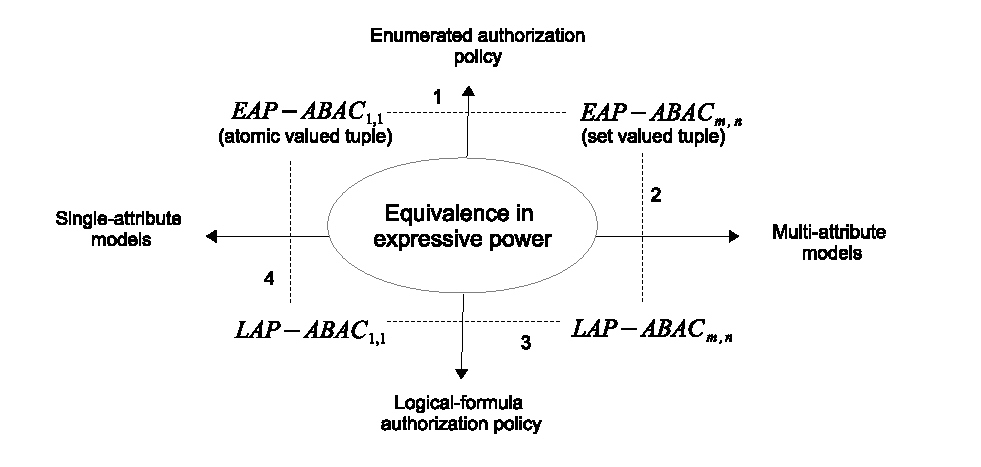
\includegraphics[width=.9\textwidth]{DBSEC16/all-equivalence}
 		\caption{Equilavence of enumerated and logical-formula auth. policy ABAC models}
 		\label{fig:all-equivalence}
 	\end{figure}
 

	 \LPMN{} (given in Figure \ref{fig:lp-abacmn-diagram}) is very similar to \EPMNModel{}, except it is based on LAPs.  It has an unbounded set of users, objects and sessions and a finite set of user attributes, object attributes, session attributes and authorization policies. \LPMN{} does not define an concrete policy language. Instead, it defines  authorization policies as any boolean function that takes values of $m$ subject and $n$ object attributes as parameters. If attribute values of a requesting subject, and requested object evaluate the authorization function $f_a$ (defined for action $a \in A$) true, corresponding access is granted. The formal definition of the model is given in Table \ref{tab:lp-abacmn-definition}. We deliberately maintain similar sets and relations (compare to \EPMNModel{})  to assert that these models only differ in the definition of authorization policies. 
	 

	

\chapter{EAP-ABAC vs LAP-ABAC in expressive power}
\label{sec:beyond}
In practice, usefulness of an access control system depends on many other aspects beyond its expressive power. For example, in the NIST special publication \textit{Guidelines  for Access Control System Evaluation Metrics} \cite{access-control-evaluation}, the authors divide these aspects into four categories including (i) administration, (ii) enforcement, (iii) performance and (iv) support. In this section, we mostly focus on administrative properties. We compare the aforementioned models from two perspectives - single attribute vs multi-attribute and enumerated vs logical-formula authorization policy.

\subsection{Single attribute vs multiple attributes}

We have seen earlier that \EPOneOneModels{} is equivalent to \EPMNModel{} and \LPOneOne{} is equivalent to \LPMN{}. But, in practice this may not be useful because of many reasons including the following.

\textbf{Attribute-value assignments and administration.} Ranges of each attribute intrinsically separate their values. For example, if \textit{role} and \textit{location} are two different attributes, values of these attributes are inherently distinguished. As a result, attribute-value assignments to users and objects and administration of these values (add or remove existing values) can be separated using semantics of individual attributes.

\textbf{Privacy concern.} If we combine values of  more than one attributes into single attribute values, a user may expose more credential than required in a particular context.  For example, combining values \textit{role} and \textit{location}, we may create values \{\textit{manager@campus, manager@home}\}. If so, a user cannot hide role  when the context requires only his location.



 \newcommand{\highlight}[1]{%
 	\colorbox{black!19}{$\displaystyle#1$}}
 
\begin{table}
	\centering
	\caption{ Different representations of  $Auth_{read}$ policy  ($Auth_{read}$ states that \textit{\manager} can access \textit{TS} objects being from either \textit{office} or \textit{home})} 
	\label{tab:LAP-heterogeneity}
	\begin{tabular}{|l|}						
		\hline					
			
			(i) $  \manager \in role(u) \land (office \in location(u) \highlight {\lor home \in location(u)})  \land TS \in sensitivity(o)$ \\
			(ii) $((\manager \in role(u) \land office \in location(u) ) \highlight {\lor (\manager \in role(u) \land home \in location(u) )}  )$ \\ \hfill $ \land TS \in sensitivity(o)$\\
			(iii) $((\manager \in role(u) \land office \mathbf{\in}\in location(u) \land TS \in sensitivity(o) ) \highlight{\lor}$  \\ \hfill $\highlight{((\manager \in role(u) \land home \in location(u) \land TS \in sensitivity(o) )}$ \\
		 \hline	
	\end{tabular}	

	
\end{table}


\textbf{Larger set to manage.} Combining values of more than one attribute together, we often need to manage larger set of values. For example, if there are ten possible values of \textit{role} and ten possible values of \textit{location}, by combining them we may need to manage one hundred values.  



\subsection{Enumerated vs logical-formula authorization policy}
In this section, we consider pros and cons of logical-formula and enumerated   authorization policy. Usually, logical formula   allows us powerful language construct to formulate even complicated business logic and policies in a succinct way. Logical formulas often support large number of logical and relational operators which make it easy to set up new policies. On the downside,  logical formulas impose little constraint on the structure, size or style of the authorization policy. As a result, policies are heterogeneous in nature having different sizes and styles. Even a single policy can be represented in so many ways.  For example, Table \ref{tab:LAP-heterogeneity} shows how a policy $Auth_{read}$ can  be represented in different three forms. The heterogeneity across multiple policies and lack of a canonical form make it difficult to understand, update or administer existing policies.  For example, to update $Auth_{read}$ so that \textit{manager} no longer gets access from \textit{home}, different representations of the policy need to be updated in different ways. Required changes to policies are highlighted in Table \ref{tab:LAP-heterogeneity}. These changes require  manual effort  by an administrator to update them. In a different aspect, LAPs are often monolithic, making it difficult to distinguish sub-policies.




On the other hand, enumerated authorization policies (EAPs), have a distinct form of representation. Thus, in \EPModels{} models, policies are homogeneous and  sub policies in a policy can be presented in one or more tuples and a  policy is a set of such tuples. Different tuples are distinguishable from each other and can be thought of as micro-policies. Thus, policies in enumerated tuples are polylithic as opposed to monolithic in logical formula. 

%Usefulness of micro policies is further discussed in Section \ref{sec:usefulness}.

On the flip side, an EAP can be very large as it  does not allow conditional expressions. For example, the  condition \textit{$age(u) \ge 18$}, should be achieved by enumerating all possible ages greater or equal 18. Another disadvantage  is that when we add/remove attributes from the system, existing EAPs may require to be updated. 

\vspace{-1em}

\subsubsection{Administration using micro-policies}
\label{sec:usefulness}

The policy $Auth_{read}$ mentioned above can be represented using micro-policies as $\{( \{\manager\}, \{office\}, \{TS\} )$, $( \{\manager\}, \{home\}, \{TS\} )\}$. In order to update the policy so that \textit{manager} can no longer access from \textit{home}, we can remove the second tuple resulting $Auth_{read} \equiv \{( \{\manager\}, \{office\}, \{TS\} )\}$. Similarly, we can add new micro-policies adding new tuples to $Auth_{read}$.

Thus, in term of administration, the minimum administrative units in EAP are micro-policies represented by policy tuples. So, it is possible that an EAP can be managed by multiple administrators at the most fine grained level of micro-policies. Design of an administrative model to manage micro-policies is beyond the scope of this paper. We postulate that as policy update can be done by merely adding or removing policy tuples,  it can be done programmatically  in \EPModels{} model. Figure \ref{fig:policy-pros-cons} shows pros and cons of \EPModels{} and \LPModels{} models. Table \ref{tab:pros-cons-table} presents a detailed comparison.




\vspace{-1em}


\subsubsection{Canonicalization of enumerated authorization policy}

In this section, we show how we can represent EAPs in a canonical form. Consider, $Auth_{write} \equiv \{( \{\manager\}, \{TS\} )$, $ ( \{\manager, dir\}, \{TS\} )\}$ in $EP$-$ABAC_{1,1}$. The first tuple says someone who is at least manager (can additionally have any other roles) can write \textit{TS} objects. The second tuple says someone both manager \& director (may additionally have any other roles) can write \textit{TS} objects. Thus, the first tuple also includes authorization requirements of the second tuple. So, if we update $Auth_{write}$ to remove the second tuple,  effectively updated $Auth'_{write}$ also represents the old policy. Thus, an enumerated authorization  policy can be represented in more than one ways which violates uniqueness of the canonical form. The advantage of representing policies in canonical form is that we make sure by adding or removing tuples, we really update the policy.  This would help  in the automation of policy administration. 


% It authorizes a \textit{manager } to access \textit{TS} objects from  \textit{office}. If the same \textit{manager} additionally holds a \textit{director} role, $Auth_{read}$ also authorizes him. This is because the authorization function checks if the requester at least (not exactly) possesses the values specified in the tuple.  Thus, if  we update $Auth_{read}$ to add a new tuple $(\{manager, director\}, \{office\}, \{TS\})$, the updated policy semantically represents the same old policy. (because the new tuple is subsumed by another tuple in the policy). Thus, an EAP can be represented in more than one forms which violets uniqueness of canonical form. 


 	\begin{figure} 
 		\centering
 		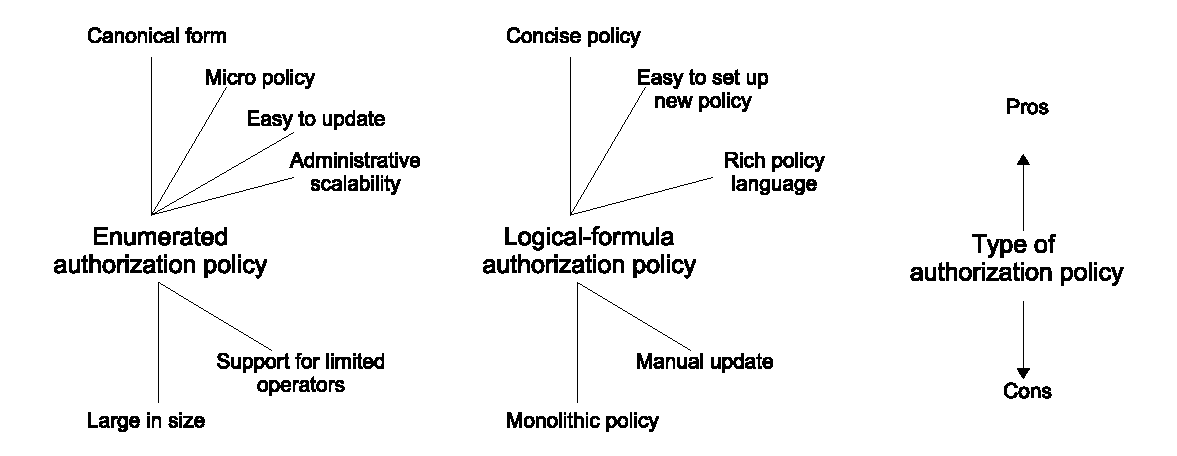
\includegraphics[width=.9\textwidth]{DBSEC16/policy-pros-cons}
 		\caption{Pros and cons of enumerated and logical-formula authorization policy}
 		\label{fig:policy-pros-cons}
 	\end{figure}

\begin{table}[]
\centering
\caption{Comparison of  LAP  and  EAP }
\label{tab:pros-cons-table}
\begin{tabular}{|c|c|c|}
	\hline
Characteristics    of   &  \begin{tabular}[c]{@{}l@{}} LAPs  (considering \\ $ABAC_\alpha$/HGABAC)  \end{tabular}     & \begin{tabular}[c]{@{}l@{}}  EAPs  (value enumeration \\ for  positive attribute-values) \end{tabular}        \\ \hline
\multicolumn{3}{l}{} \\ 
\multicolumn{3}{l}{\textit{\textbf{Definition}}} \\ \hline
\begin{tabular}[c]{@{}l@{}} \textit{distinguishing features}\end{tabular} & \begin{tabular}[c]{@{}l@{}}  logical-formula \end{tabular} & \begin{tabular}[c]{@{}l@{}}  enumeration\end{tabular} \\ \hline
\multicolumn{3}{l}{} \\ 
\multicolumn{3}{l}{\textit{\textbf{Syntax}}} \\ \hline

\begin{tabular}[c]{@{}l@{}}\textit{Representation} \end{tabular} & \begin{tabular}[c]{@{}l@{}} expression \end{tabular} & \begin{tabular}[c]{@{}l@{}} set  \end{tabular} \\ \hline

\begin{tabular}[c]{@{}l@{}}\textit{Morphism} \end{tabular} & \begin{tabular}[c]{@{}l@{}} polymorphic (single policy can \\  be represented many ways) \end{tabular} & \begin{tabular}[c]{@{}l@{}} unique representation \end{tabular} \\ \hline

\begin{tabular}[c]{@{}l@{}}\textit{Policy type}\end{tabular} & \begin{tabular}[c]{@{}l@{}} macro-policy, \\ possibly cohesive sub-policies\end{tabular} & \begin{tabular}[c]{@{}l@{}} micro-policy, \\ disjointed sub-policies  \end{tabular} \\ \hline

\begin{tabular}[c]{@{}l@{}}\textit{Divisibility}\end{tabular} & \begin{tabular}[c]{@{}l@{}} monolithic\end{tabular} & \begin{tabular}[c]{@{}l@{}} polylithic  \end{tabular} \\ \hline


\begin{tabular}[c]{@{}l@{}}\textit{Size}\end{tabular} & \begin{tabular}[c]{@{}l@{}} usually concise\end{tabular} & \begin{tabular}[c]{@{}l@{}}  usually large  \end{tabular} \\ \hline

\begin{tabular}[c]{@{}l@{}}\textit{Language}\end{tabular} & \begin{tabular}[c]{@{}l@{}} propositional/ \\ first-order logic formula\end{tabular} & \begin{tabular}[c]{@{}l@{}} equivalent to DNF \\  of logical formula  \end{tabular} \\ \hline

 
 \multicolumn{3}{l}{} \\ 
 \multicolumn{3}{l}{\textit{\textbf{Semantics}}} \\ \hline
 
 \begin{tabular}[l]{@{}l@{}}\textit{Set of granted  privileges} \end{tabular} & \begin{tabular}[c]{@{}l@{}} dynamic (may change on addition/ \\removal  of attribute-values)\end{tabular} & \begin{tabular}[c]{@{}l@{}}static (privilege is explicitly\\ granted) \end{tabular} \\ \hline 


 \begin{tabular}[c]{@{}l@{}}\textit{Required attribute-value }\\ \textit{assgnments for granting} \\ \textit{privileges} \end{tabular} & \begin{tabular}[c]{@{}l@{}} partial assignments may \\  grant privilege\end{tabular} & \begin{tabular}[c]{@{}l@{}} requires complete assignment  \end{tabular} \\ \hline 
 
% \begin{tabular}[c]{@{}l@{}}\textit{ Privilege abstraction} \end{tabular} & \begin{tabular}[c]{@{}l@{}} may abstract granted privileges\end{tabular} & \begin{tabular}[c]{@{}l@{}} no privilege abstraction  \end{tabular} \\ \hline 

\multicolumn{3}{l}{} \\ 
\multicolumn{3}{l}{\textit{\textbf{Administration}}} \\ \hline

\begin{tabular}[c]{@{}l@{}}\textit{Cost of reviewing policy} \end{tabular} & \begin{tabular}[c]{@{}l@{}} NP-complete \end{tabular} & \begin{tabular}[c]{@{}l@{}} polynomial \\ (in number of tuples) \end{tabular} \\ \hline

%\multicolumn{3}{l}{\textit{\textbf{Privilege administration}}} \\ \hline

\begin{tabular}[c]{@{}l@{}}\textit{Granting new privilege} \end{tabular} & \begin{tabular}[c]{@{}l@{}} manual update \end{tabular} & \begin{tabular}[c]{@{}l@{}} add new tuples \end{tabular} \\ \hline

\begin{tabular}[c]{@{}l@{}}\textit{Remove existing privileges} \end{tabular} & \begin{tabular}[c]{@{}l@{}}manual update  \end{tabular} & \begin{tabular}[c]{@{}l@{}} remove tuples \end{tabular} \\ \hline 

\begin{tabular}[c]{@{}l@{}}\textit{Minimum administrative unit} \end{tabular} & \begin{tabular}[c]{@{}l@{}} entire policy \end{tabular} & \begin{tabular}[c]{@{}l@{}} micro-policy \end{tabular} \\ \hline   

\begin{tabular}[c]{@{}l@{}}\textit{scalability} \end{tabular} & \begin{tabular}[c]{@{}l@{}} not scalable  \end{tabular} & \begin{tabular}[c]{@{}l@{}} \hfil scalable \end{tabular} \\ \hline     

\multicolumn{3}{l}{} \\ 
\multicolumn{3}{l}{\textit{\textbf{Application}}} \\ \hline

\begin{tabular}[l]{@{}l@{}}\textit{} Convenient for \end{tabular} & \begin{tabular}[c]{@{}l@{}} specifying new policy, \\  administration using range \\ of attribute-values\end{tabular} & \begin{tabular}[c]{@{}l@{}}  updating policy, \\ fine grained administration\end{tabular} \\ \hline 

\begin{tabular}[l]{@{}l@{}}\textit{} Suitable environment \end{tabular} & \begin{tabular}[c]{@{}l@{}} open, loosely administered system, \\ distributed administration\end{tabular} & \begin{tabular}[c]{@{}l@{}}  close, tightly administered \\ system\end{tabular} \\ \hline 

                                        
\end{tabular}
\end{table}

To represent \EAP{}s in a canonical form, we ensure that in the same policy, no policy-tuple subsumes another policy-tuple. Formally, let $t_i$ denotes $i^{th}$ tuple in a policy and $S_{ik}$  be the $k^{th}$ set in tuple $t_i$. We say, a policy tuple $t_i$ subsumes $t_j$ iff  $(\exists p \in \{1,2,..,m+n\}, \forall q \in \{1,2,..,m+n\} \setminus {p})[S_{ip} \subseteq S_{jp} \land (S_{iq} \subseteq S_{jq} \lor S_{ip} = S_{jp}) ]$. For example, for $t1=(\{\manager,dir\}, \{TS\})$,$t2=(\{\manager, dir, adv\}, \{TS\})$, $t3=(\{\manager,dir, adv\}, \{H\})$ t1 includes t2 but none of t1 and t2 includes t3. 



To maintain a canonical representation of EAPs, we can remove policy-tuples that have been subsumed by other tuples. It is also possible to specify more sophisticated meta policies to manage subsumed policy-tuples.  




\section{Related work}
\label{sec:related-work}
	%\subsection{Related work}

	Several attribute based access control models have been proposed in the literature. Most of them are based on logical-formula authorization policies. For example,	$\abacAlpha{}$ \cite{abacAlpha} is among the first few models to formally define an ABAC model.  $\abacAlpha{}$ was developed  for the specific purpose of simulating simple forms of DAC, MAC and RBAC policies. As such, it deliberately has a more restrictive (and less powerful) policy language.  On the other hand, $\hgabac{}$ \cite{hgabac} is more general in purpose and also capable of accommodating  the traditional models. Both $\abacAlpha{}$ and \hgabac{} use propositional logic as their policy language. In the very same direction, ABAC-for-web-services \cite{abac-for-web-service} is among very few earlier works to outline authorization architecture and policy formulation for an ABAC system. Other notable work for the development of logical formula ABAC model include \cite{grid-abac,ontologies,abac-ws,wang2004logic}.
	
    NIST ABAC guide \cite{nist-abac-draft} and other publications \cite{hu2015attribute}  are also significant in defining concepts, required components, considerations and architecture for designing an  enterprise ABAC system. They acknowledge the fact that ABAC rules can be quite complex in boolean combination of attributes or in simple relations involving attributes.    
    
%    It is designed to demonstrate flexibilities of an ABAC system to configure DAC, MAC and RBAC models. As such,
    
	%In the other direction, Policy Machine (PM) \cite{policy-machine} and \labac{} \cite{labac} are	examples of ABAC models based on enumerated authorization policy. A policy/privilege in PM is defined as $(ua_i, OP, oa_i)$, where $ua_i$ and $oa_i$ are values of user-attribute and object-attribute respectively and $OP$ is  a set of operations. A policy tuple in \labac{} is also defined a very similar way specified as $(user\_attr\_value, action, object\_attr\_value)$. Both of these two models have also demonstrate their flexibility in configuring traditional models in it. In a very similar way, authorization policies is enumerated in \twoSortedRBAC{} \cite{two-sorted-rbac} in the  context of role.  
	
	Damiani et al \cite{damiani2005} describe an informal framework for 	attribute based access control in open environments. Bonatti et al \cite{bonatti,bonatti2} present a uniform structure to logically formulate and reason about both service access and information disclosure constraints according to related entity attributes. 	
	
	Other related work include XACML \cite{xacml}, UCON \cite{ucon}, policy mining \cite{mining},attribute certificates \cite{attribute-cert} and so on \cite{enforcing,lee,foley}.
	
	 %ABE \cite{abe} 
	%Similarly, [28,29,30] develop a service negotiation framework for requesters and providers to gradually expose their attributes.

	 %XACML \cite{xacml} is a declarative access control policy language and processing model which  supports attribute based concepts and policies. Although, it lacks a formal definition of an ABAC model, it is notable for its uses in multiple commercial products.
	 

\section{Conclusion}
\label{sec:conclusion}
%Logical-formulas and enumerated  tuples are two major ways to specify authorization policies in an ABAC model.  In this paper, we show that they are equivalent in theoretical expressive power. We also analyze these models beyond their expressive power. We show that logical-formulas are flexible and convenient for setting up new authorization  policies but they are difficult to update/administer policies. On the other hand, enumerated authorization policies can be difficult to set up by enumerating all possible tuples but they are convenient for policy update and administration. We further show usefulness of enumerated policies by demonstrating how it supports micro policies and how it can be extended to be represented in a canonical form. 

In this paper, we present a finite attribute finite domain ABAC model using enumerated authorization policies. We then compare enumerated authorization policy ABAC models (\EPModels) with logical-formula authorization policy ABAC (\LPModels) models in finite domain. We show that they are equivalent in term of theoretical expressive power. We also analyze these models beyond their expressive power. While, logical-formulas are flexible and convenient for setting up new authorization  policies, enumeration is convenient for updating or administering policies. We also show that enumerated authorization policies facilitate micro-policies and can easily be represented in a canonical form. Canonical representation and support for micro policies enable automated and scalable administration. 

%Micro policies along with its canonical representation can help in automated and scalable administration. 

%A natural question to ask how we can take advantage of both approaches so that both specification of new policies and administration of existing policies are convenient. Can we combine enumerated and logical formula policies? Can we canonicalize logical formulas and take advantage in policy administration? Further research is also required to better understand micro policies and canonicalization of authorization policies. 

%* Connect with Ninguili's ARBAC evaluation perspectives.
%%\vspace{-1em}
\renewcommand{\suffix}{m,n}
\newcommand{\suffixT}{1,1}
\begin{table}
	\centering
	\caption{ Mappings } %\vspace*{3pt}
	\label{tab:lp11-to-lpmn}
	\begin{tabular}{|l|}						
		\hline					
%			\multicolumn{1}{|c|}{\underline{\textit{I. \LPOneOne{} components}}} \\
%				  - $U, O, A, S, UAV, OAV$  (users,  objects, actions, subjects, user and object attr. values.)\\
%				  - $ua,oa$ (attribute functions);  $ua:U\to 2^{UAV}$; $oa:O\to 2^{OAV}$ \\ 
%				  - $\subCreator: S \to U$ ; $sa:S\to 2^{UAV}$,    $sa(s) \subseteq ua(\subCreator(s))$\\
%				  - $f_a: (sa(u), oa(o)) \to \{true, false\}$  and $\isAuthorized(s,a,o) =(f_a(sa(u),oa(o))=true$) \\
				 
		   
		   \multicolumn{1}{|c|}{\underline{\textit{I. From \LPMN{} to \LPOneOne{}}}}\\	
			   - $U = U_{\suffix}; O = O_{\suffix}; A = A_{\suffix}; S = S_{\suffix};$$\textit{UAV} = \UAV{1} \times \UAV{2}\times ... \times \UAV{m}$\\
			   -  $\textit{OAV} = \OAV{1} \times \OAV{2}\times ... \times \OAV{m}$;$ua(u) = \ua{1}(u) \times \ua{2}(u) \times ... \times \ua{m}(u) $\\
			   -$oa(u) = \oa{1}(u) \times  ... \times \oa{m}(u) $$sa(u) = \sa{1}(u) \times ... \times \sa{m}(u) $; $\creator(s) = \creator_{\suffix}(s)$\\
			    - $ f_a =$ $\mathop{\bigvee}\limits_{ f_{a_{m,n}}( \ULS{1}, \ULS{2},...\ULS{m}, \OLS{1}, \OLS{2}, ...,\OLS{n})=true }  (\ULS{1}(u) \times ... \times \ULS{m}(u) \subseteq ua(u) )\land$ \\ \hfill  $(\OLS{1}(o) \times ... \times \OLS{n}(o) \subseteq oa(o))$, for $\ULS{i} \subseteq \UAV{i}$ and $\OLS{i} \subseteq \OAV{i}$ \\ 		
			   
 
	   \multicolumn{1}{|c|}{\underline{\textit{II. From \LPOneOne{} to \LPMN{}}}}\\	
			- $U = U_{\suffixT}; O = O_{\suffixT}; A = A_{\suffixT}; S = S_{\suffixT};$\\
			- $\UAV{1} = UAV; \UAV{2} = \{\}; ... \UAV{m} = \{\};$  $\OAV{1} = OAV; \OAV{2} = \{\}; ... \OAV{n} = \{\};$\\
			- $\ua{1}(u) = ua(u); \ua{2}(u) = \{\};...\ua{m}(u) = \{\}$; $\oa{1}(o) = oa(o); \oa{2}(o) = \{\};...\oa{m}(o) = \{\}$\\
		    - $\sa{1}(u) = sa(u); \sa{2}(u) = \{\};...\sa{m}(u) = \{\}$; $\creator_{\suffix}(s) = \creator(s)$ and $f_{a_{\suffix}} =$\\
		    $\mathop{\bigvee}\limits_{ f_{a}( \ULS{i},\OLS{i})=true }  (\ULS{i} \subseteq \ua{1}(u) \land$   $ \OLS{i}\subseteq oa(o))$  for $\ULS{i} \subseteq UAV$ and $\OLS{i} \subseteq OAV$ \\ 
		 %\hline	
		 	\multicolumn{1}{|c|}{\underline{\textit{III. From \EPOneOneModels{} to \LPOneOne{} }}}\\					
		 	- $U  = U ; O  = O ; A  = A $; $UAV	= UL; OAV = OL$;$ua(u) = uLabel(u)$; $oa(o)=oLabel(o) $\\
		 	-  $sa(s) = \sessionLabels(s) $ ;$f_a =$ $\mathop{\vee}\limits_{ (ul_i, ol_i) \in \policy_a} ( ul_i \in ua(u) \land ol_i \in oa(o))$. \\
		 	
		 	\multicolumn{1}{|c|}{\underline{\textit{IV. From \LPOneOne{} to \EPOneOneModels{}}}}\\	
		 	- $UL= 2^{ULV}; OL= 2^{OLV}; \uLabel(u) = 2^{ua(u)};\oLabel(o) = 2^{oa(o)}; \sessionLabels(s) = 2^{sa(s)}$ \\	  
		 	- $\Policy_a = \{  (\ulsubset, \olsubset) | (\exists \ulsubset \subseteq UL, \exists \olsubset \subseteq OL)[ f_a(\ulsubset, o\ulsubset) = true] \} $
		 	
		 	\\ \hline	
	\end{tabular}	

	
\end{table}
%\vspace{-1.5em}












%%\vspace{-1em}
\renewcommand{\denom}{0}
\renewcommand{\suffix}{0}
\renewcommand{\suffixTwo}{0}
\begin{table}
	\centering
	\caption{ Mapping from \clabac{} to \EPMNModel{}  } %\vspace*{3pt}
	\label{tab:mapping-clabac-to-slabac}
	\begin{tabular}{|l|}						
		\hline					
			\multicolumn{1}{|c|}{\underline{\textit{I. \clabac{} components}}} \\
			-  $U_\suffix, O_\suffix,  A_\suffix, S_\suffix, UL_\suffix$, $OL_\suffix$ (users, objects, actions, sessions, $uLabel$ and $oLabel$ values resp.) \\ 				  
			-  $\uLabel_\suffix: U_\suffix \to 2^{UL_\suffix}$, $\oLabel_\suffix: O_\suffix \to 2^{OL_\suffix}$; $\creator_\suffix: S_\suffix \to U_\suffix$; $\sessionLabels_\suffix: S_\suffix \to 2^{UL_\suffix}$ \\
			- $\Policy_a \subseteq 2^{UL_\suffix} \times 2^{OL_\suffix}$ and $\Policy_\suffix = \{Policy_a | a \in A\}$\\
		   
	 \multicolumn{1}{|c|}{\underline{\textit{II. Construction}}}\\	
			- $U = U_\denom, O = O_\denom, A = A_\denom, S_\suffixTwo = S$ \\
			- $\UL{1} = \UL{0}$, $\UL{i} = \{\}$, for $2\le i \le m$\\
			- $\OL{1} = \OL{0}$, $\OL{i} = \{\}$, for $2\le i \le n$\\
			- $\uLabelP{1}(u) = \uLabelP{0}(u)$, $\uLabelP{i}(u) = \{\}$, for $2 \le i  \le m $\\
			- $\oLabelP{1}(o) = \oLabelP{0}(u)$, $\oLabelP{i}(o) = \{\}$, for $2 \le i  \le n $\\
			- $\creator_0(s) = \creator(s)$, for $s \in S$\\
			- $\sessionLabelsP{1}(s) = \sessionLabelsP{0}(s)$, $\sessionLabelsP{i}(s) = \{\}$, for $2 \le i \le m$\\
			- $\Policy_a = \{( \{ul\}, \{\}, ...\{\}, \{ol\}, \{\}, ... \{\} ) | (ul,ol) \in \Policy_a[ \Policy_a \in \Policy_\suffix]\}$\\
		 \hline	
	\end{tabular}	

	
\end{table}
%\vspace{-1em}
We acknowledge an error found in the authorization function of the  \EPMNModel{} model as found in Table 1  of 4th page of this paper. The updated definition of the authorization function (with corrections highlighted) is presented below. \\

$is\_authorized(s:S, a:A, o:O) = (\exists (ULS_1,ULS_2, ..., ULS_m, OLS_1,$ \\$ OLS_2, ... OLS_n ) $ 
$ \in Policy_a)[ULS_i \highlight{=} sLabel_i(s), \text{for } 1 \le i \le m \land$  \\ \hfill $ \OLS{i} \highlight{=} oLabel{i}(o), \text{for } 1 \le i \le n]$ 

\bibliographystyle{abbrv}
\bibliography{sigproc}
\vspace{-2em}


\end{document}
